\documentclass[a4paper,11pt,titlepage]{article}
\usepackage{graphicx}
\author{Abrie Greeff\\B.Sc Hons (Computer Science)\\Department of Computer Science\\University of Stellenbosch}
\title{Self Organising Maps}
\begin{document}
\maketitle
\tableofcontents

\section{Question 1}
This application was developed in Java. The assumption was made that the sample data would always be three-dimensional. This enabled me to use the sample data as a colour vector. Colour vectors consist of three components the red, green and blue intensity values.

When a weight was chosen to be nearest to a randomly chosen sample, the Euclidean distance was computed to determine the nearest weight. A Gaussian function as in \cite{web1} was computed to determine the neighbours and the level of interaction they have with the sample data. Scaling was also done using the formula described in \cite{web1}.

The application generates an initial random data set. It is then trained using a provided sample set. The application has two output windows. The first is the map represented by colours and the second is a U-Map used to compare differences in gradient. This interface can be seen in Figure~\ref{Figure:gui}.

To execute this application type \emph{java SOM} in your console. This will provide you with all the necessary command line parameter options.

\begin{figure}[htbp]
   \centering
   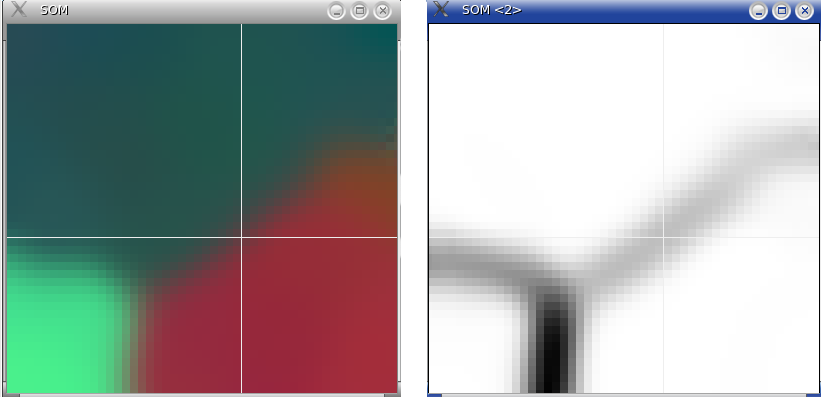
\includegraphics[width=9cm]{gui.png}
   \caption{Application Interface}
   \label{Figure:gui}
\end{figure}

\section{Question 2}
This application is used to randomly generate 50000 colour vectors. Six reference vectors is randomly created. Every vector is assigned a random portion of the 50000 points. Random noise is added to each reference vector to create deviations of the reference vector. All of these points are then saved to an output file to be used as a sample data set.

To execute this application type \emph{java random file} in your console, where \emph{file} is the name of the generated sample data file.

\section{Question 3}
The first thing I did for this question was to generate a data set of 50000 points using the application developed in Question 2. This data set was then used to train a self organising map (SOM). The application used to train on was the application developed for Question 1. A 50x50 grid was created with initial random vector points and 100000 iterations was run.

After all iterations were done the SOM output was reached as in Figure~\ref{Figure:som}. The U-Map output for this iterations is given in Figure~\ref{Figure:umap}.


\begin{figure}[htbp]
   \centering
   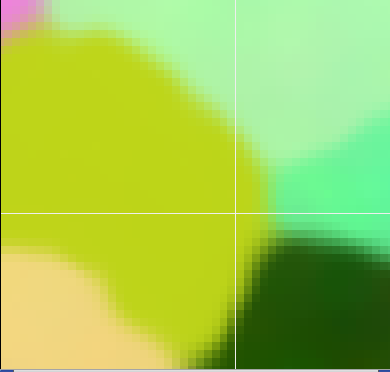
\includegraphics[width=9cm]{som.png}
   \caption{Self Organising Map}
   \label{Figure:som}
\end{figure}

\begin{figure}[htbp]
   \centering
   
\includegraphics[width=9cm]{umap.png}
   \caption{U-Map}
   \label{Figure:umap}
\end{figure}


\section{Question 4}
An possible extension to the SOM application could be to add the capabilities to classify data. The purpose of this question is to investigate this and try to implement the extension. After considering many possibilities I decided on an extension.

The problem was what distinguishes data from each other and makes them similar. To choose a way to store each set of data before being classified I also had to remember to stay with the way SOMs store data. Finally I chose to represent each set of data as a vector. To do this every character in an input file was saved as a coordinate of a vector corresponding to this file. This means if a file contained 16 characters the vector size would be 16.

All the files needed to train the classifier is then loaded into their respective vectors and given a position in the map. The test data is then loaded into their respective vectors and by using the Euclidean distance the nearest vector in the training data is then computed. The test vector is then classified to be the nearest to this vector.
\subsection{Facial Recognition}
To test this extension \emph{SOM.java} was modified to be a facial recognition application. This application can be executed by typing \emph{java SOMface} in the console. I trained this program on 280 faces, where every set of seven was from the same person. I then tried to classify 80 pictures, where every set of two pictures corresponded to a set in the training data. I achieved a success rate of 58\% with this set of data. Which was excellent considering the quality of the data. A sample training file is provided in \emph{test}. Below is the output generated by the program.

\begin{verbatim}
java SOMface -d -s train
Loading sample data
Loading./database/1/lowres16/1lr.int
Loading./database/1/lowres16/2lr.int
Loading./database/1/lowres16/3lr.int
Loading./database/1/lowres16/4lr.int
Loading./database/1/lowres16/5lr.int
Loading./database/1/lowres16/6lr.int
Loading./database/1/lowres16/7lr.int
Loading./database/1/lowres16/8lr.int
Loading./database/1/lowres16/9lr.int
Loading./database/2/lowres16/1lr.int
Loading./database/2/lowres16/2lr.int
Loading./database/2/lowres16/3lr.int
Loading./database/2/lowres16/4lr.int
Loading./database/2/lowres16/5lr.int
Loading./database/2/lowres16/6lr.int
Loading./database/2/lowres16/7lr.int
Loading./database/2/lowres16/8lr.int
Loading./database/2/lowres16/9lr.int
Loading./database/3/lowres16/1lr.int
Loading./database/3/lowres16/2lr.int
Loading./database/3/lowres16/3lr.int
Loading./database/3/lowres16/4lr.int
Loading./database/3/lowres16/5lr.int
Loading./database/3/lowres16/6lr.int
Loading./database/3/lowres16/7lr.int
Loading./database/3/lowres16/8lr.int
Loading./database/3/lowres16/9lr.int
Loading./database/4/lowres16/1lr.int
Loading./database/4/lowres16/2lr.int
Loading./database/4/lowres16/3lr.int
Loading./database/4/lowres16/4lr.int
Loading./database/4/lowres16/5lr.int
Loading./database/4/lowres16/6lr.int
Loading./database/4/lowres16/7lr.int
Loading./database/4/lowres16/8lr.int
Loading./database/4/lowres16/9lr.int
Loading./database/5/lowres16/1lr.int
Loading./database/5/lowres16/2lr.int
Loading./database/5/lowres16/3lr.int
Loading./database/5/lowres16/4lr.int
Loading./database/5/lowres16/5lr.int
Loading./database/5/lowres16/6lr.int
Loading./database/5/lowres16/7lr.int
Loading./database/5/lowres16/8lr.int
Loading./database/5/lowres16/9lr.int
Loading./database/6/lowres16/1lr.int
Loading./database/6/lowres16/2lr.int
Loading./database/6/lowres16/3lr.int
Loading./database/6/lowres16/4lr.int
Loading./database/6/lowres16/5lr.int
Loading./database/6/lowres16/6lr.int
Loading./database/6/lowres16/7lr.int
Loading./database/6/lowres16/8lr.int
Loading./database/6/lowres16/9lr.int
Loading./database/7/lowres16/1lr.int
Loading./database/7/lowres16/2lr.int
Loading./database/7/lowres16/3lr.int
Loading./database/7/lowres16/4lr.int
Loading./database/7/lowres16/5lr.int
Loading./database/7/lowres16/6lr.int
Loading./database/7/lowres16/7lr.int
Loading./database/7/lowres16/8lr.int
Loading./database/7/lowres16/9lr.int
Loading./database/8/lowres16/1lr.int
Loading./database/8/lowres16/2lr.int
Loading./database/8/lowres16/3lr.int
Loading./database/8/lowres16/4lr.int
Loading./database/8/lowres16/5lr.int
Loading./database/8/lowres16/6lr.int
Loading./database/8/lowres16/7lr.int
Loading./database/8/lowres16/8lr.int
Loading./database/8/lowres16/9lr.int
Loading./database/9/lowres16/1lr.int
Loading./database/9/lowres16/2lr.int
Loading./database/9/lowres16/3lr.int
Loading./database/9/lowres16/4lr.int
Loading./database/9/lowres16/5lr.int
Loading./database/9/lowres16/6lr.int
Loading./database/9/lowres16/7lr.int
Loading./database/9/lowres16/8lr.int
Loading./database/9/lowres16/9lr.int
Loading./database/10/lowres16/1lr.int
Loading./database/10/lowres16/2lr.int
Loading./database/10/lowres16/3lr.int
Loading./database/10/lowres16/4lr.int
Loading./database/10/lowres16/5lr.int
Loading./database/10/lowres16/6lr.int
Loading./database/10/lowres16/7lr.int
Loading./database/10/lowres16/8lr.int
Loading./database/10/lowres16/9lr.int
Loading./database/11/lowres16/1lr.int
Loading./database/11/lowres16/2lr.int
Loading./database/11/lowres16/3lr.int
Loading./database/11/lowres16/4lr.int
Loading./database/11/lowres16/5lr.int
Loading./database/11/lowres16/6lr.int
Loading./database/11/lowres16/7lr.int
Loading./database/11/lowres16/8lr.int
Loading./database/11/lowres16/9lr.int
Loading./database/12/lowres16/1lr.int
Loading./database/12/lowres16/2lr.int
Loading./database/12/lowres16/3lr.int
Loading./database/12/lowres16/4lr.int
Loading./database/12/lowres16/5lr.int
Loading./database/12/lowres16/6lr.int
Loading./database/12/lowres16/7lr.int
Loading./database/12/lowres16/8lr.int
Loading./database/12/lowres16/9lr.int
Loading./database/13/lowres16/1lr.int
Loading./database/13/lowres16/2lr.int
Loading./database/13/lowres16/3lr.int
Loading./database/13/lowres16/4lr.int
Loading./database/13/lowres16/5lr.int
Loading./database/13/lowres16/6lr.int
Loading./database/13/lowres16/7lr.int
Loading./database/13/lowres16/8lr.int
Loading./database/13/lowres16/9lr.int
Loading./database/14/lowres16/1lr.int
Loading./database/14/lowres16/2lr.int
Loading./database/14/lowres16/3lr.int
Loading./database/14/lowres16/4lr.int
Loading./database/14/lowres16/5lr.int
Loading./database/14/lowres16/6lr.int
Loading./database/14/lowres16/7lr.int
Loading./database/14/lowres16/8lr.int
Loading./database/14/lowres16/9lr.int
Loading./database/15/lowres16/1lr.int
Loading./database/15/lowres16/2lr.int
Loading./database/15/lowres16/3lr.int
Loading./database/15/lowres16/4lr.int
Loading./database/15/lowres16/5lr.int
Loading./database/15/lowres16/6lr.int
Loading./database/15/lowres16/7lr.int
Loading./database/15/lowres16/8lr.int
Loading./database/15/lowres16/9lr.int
Loading./database/16/lowres16/1lr.int
Loading./database/16/lowres16/2lr.int
Loading./database/16/lowres16/3lr.int
Loading./database/16/lowres16/4lr.int
Loading./database/16/lowres16/5lr.int
Loading./database/16/lowres16/6lr.int
Loading./database/16/lowres16/7lr.int
Loading./database/16/lowres16/8lr.int
Loading./database/16/lowres16/9lr.int
Loading./database/17/lowres16/1lr.int
Loading./database/17/lowres16/2lr.int
Loading./database/17/lowres16/3lr.int
Loading./database/17/lowres16/4lr.int
Loading./database/17/lowres16/5lr.int
Loading./database/17/lowres16/6lr.int
Loading./database/17/lowres16/7lr.int
Loading./database/17/lowres16/8lr.int
Loading./database/17/lowres16/9lr.int
Loading./database/18/lowres16/1lr.int
Loading./database/18/lowres16/2lr.int
Loading./database/18/lowres16/3lr.int
Loading./database/18/lowres16/4lr.int
Loading./database/18/lowres16/5lr.int
Loading./database/18/lowres16/6lr.int
Loading./database/18/lowres16/7lr.int
Loading./database/18/lowres16/8lr.int
Loading./database/18/lowres16/9lr.int
Loading./database/19/lowres16/1lr.int
Loading./database/19/lowres16/2lr.int
Loading./database/19/lowres16/3lr.int
Loading./database/19/lowres16/4lr.int
Loading./database/19/lowres16/5lr.int
Loading./database/19/lowres16/6lr.int
Loading./database/19/lowres16/7lr.int
Loading./database/19/lowres16/8lr.int
Loading./database/19/lowres16/9lr.int
Loading./database/20/lowres16/1lr.int
Loading./database/20/lowres16/2lr.int
Loading./database/20/lowres16/3lr.int
Loading./database/20/lowres16/4lr.int
Loading./database/20/lowres16/5lr.int
Loading./database/20/lowres16/6lr.int
Loading./database/20/lowres16/7lr.int
Loading./database/20/lowres16/8lr.int
Loading./database/20/lowres16/9lr.int
Loading./database/21/lowres16/1lr.int
Loading./database/21/lowres16/2lr.int
Loading./database/21/lowres16/3lr.int
Loading./database/21/lowres16/4lr.int
Loading./database/21/lowres16/5lr.int
Loading./database/21/lowres16/6lr.int
Loading./database/21/lowres16/7lr.int
Loading./database/21/lowres16/8lr.int
Loading./database/21/lowres16/9lr.int
Loading./database/22/lowres16/1lr.int
Loading./database/22/lowres16/2lr.int
Loading./database/22/lowres16/3lr.int
Loading./database/22/lowres16/4lr.int
Loading./database/22/lowres16/5lr.int
Loading./database/22/lowres16/6lr.int
Loading./database/22/lowres16/7lr.int
Loading./database/22/lowres16/8lr.int
Loading./database/22/lowres16/9lr.int
Loading./database/23/lowres16/1lr.int
Loading./database/23/lowres16/2lr.int
Loading./database/23/lowres16/3lr.int
Loading./database/23/lowres16/4lr.int
Loading./database/23/lowres16/5lr.int
Loading./database/23/lowres16/6lr.int
Loading./database/23/lowres16/7lr.int
Loading./database/23/lowres16/8lr.int
Loading./database/23/lowres16/9lr.int
Loading./database/24/lowres16/1lr.int
Loading./database/24/lowres16/2lr.int
Loading./database/24/lowres16/3lr.int
Loading./database/24/lowres16/4lr.int
Loading./database/24/lowres16/5lr.int
Loading./database/24/lowres16/6lr.int
Loading./database/24/lowres16/7lr.int
Loading./database/24/lowres16/8lr.int
Loading./database/24/lowres16/9lr.int
Loading./database/25/lowres16/1lr.int
Loading./database/25/lowres16/2lr.int
Loading./database/25/lowres16/3lr.int
Loading./database/25/lowres16/4lr.int
Loading./database/25/lowres16/5lr.int
Loading./database/25/lowres16/6lr.int
Loading./database/25/lowres16/7lr.int
Loading./database/25/lowres16/8lr.int
Loading./database/25/lowres16/9lr.int
Loading./database/26/lowres16/1lr.int
Loading./database/26/lowres16/2lr.int
Loading./database/26/lowres16/3lr.int
Loading./database/26/lowres16/4lr.int
Loading./database/26/lowres16/5lr.int
Loading./database/26/lowres16/6lr.int
Loading./database/26/lowres16/7lr.int
Loading./database/26/lowres16/8lr.int
Loading./database/26/lowres16/9lr.int
Loading./database/27/lowres16/1lr.int
Loading./database/27/lowres16/2lr.int
Loading./database/27/lowres16/3lr.int
Loading./database/27/lowres16/4lr.int
Loading./database/27/lowres16/5lr.int
Loading./database/27/lowres16/6lr.int
Loading./database/27/lowres16/7lr.int
Loading./database/27/lowres16/8lr.int
Loading./database/27/lowres16/9lr.int
Loading./database/28/lowres16/1lr.int
Loading./database/28/lowres16/2lr.int
Loading./database/28/lowres16/3lr.int
Loading./database/28/lowres16/4lr.int
Loading./database/28/lowres16/5lr.int
Loading./database/28/lowres16/6lr.int
Loading./database/28/lowres16/7lr.int
Loading./database/28/lowres16/8lr.int
Loading./database/28/lowres16/9lr.int
Loading./database/29/lowres16/1lr.int
Loading./database/29/lowres16/2lr.int
Loading./database/29/lowres16/3lr.int
Loading./database/29/lowres16/4lr.int
Loading./database/29/lowres16/5lr.int
Loading./database/29/lowres16/6lr.int
Loading./database/29/lowres16/7lr.int
Loading./database/29/lowres16/8lr.int
Loading./database/29/lowres16/9lr.int
Loading./database/30/lowres16/1lr.int
Loading./database/30/lowres16/2lr.int
Loading./database/30/lowres16/3lr.int
Loading./database/30/lowres16/4lr.int
Loading./database/30/lowres16/5lr.int
Loading./database/30/lowres16/6lr.int
Loading./database/30/lowres16/7lr.int
Loading./database/30/lowres16/8lr.int
Loading./database/30/lowres16/9lr.int
Loading./database/31/lowres16/1lr.int
Loading./database/31/lowres16/2lr.int
Loading./database/31/lowres16/3lr.int
Loading./database/31/lowres16/4lr.int
Loading./database/31/lowres16/5lr.int
Loading./database/31/lowres16/6lr.int
Loading./database/31/lowres16/7lr.int
Loading./database/31/lowres16/8lr.int
Loading./database/31/lowres16/9lr.int
Loading./database/32/lowres16/1lr.int
Loading./database/32/lowres16/2lr.int
Loading./database/32/lowres16/3lr.int
Loading./database/32/lowres16/4lr.int
Loading./database/32/lowres16/5lr.int
Loading./database/32/lowres16/6lr.int
Loading./database/32/lowres16/7lr.int
Loading./database/32/lowres16/8lr.int
Loading./database/32/lowres16/9lr.int
Loading./database/33/lowres16/1lr.int
Loading./database/33/lowres16/2lr.int
Loading./database/33/lowres16/3lr.int
Loading./database/33/lowres16/4lr.int
Loading./database/33/lowres16/5lr.int
Loading./database/33/lowres16/6lr.int
Loading./database/33/lowres16/7lr.int
Loading./database/33/lowres16/8lr.int
Loading./database/33/lowres16/9lr.int
Loading./database/34/lowres16/1lr.int
Loading./database/34/lowres16/2lr.int
Loading./database/34/lowres16/3lr.int
Loading./database/34/lowres16/4lr.int
Loading./database/34/lowres16/5lr.int
Loading./database/34/lowres16/6lr.int
Loading./database/34/lowres16/7lr.int
Loading./database/34/lowres16/8lr.int
Loading./database/34/lowres16/9lr.int
Loading./database/35/lowres16/1lr.int
Loading./database/35/lowres16/2lr.int
Loading./database/35/lowres16/3lr.int
Loading./database/35/lowres16/4lr.int
Loading./database/35/lowres16/5lr.int
Loading./database/35/lowres16/6lr.int
Loading./database/35/lowres16/7lr.int
Loading./database/35/lowres16/8lr.int
Loading./database/35/lowres16/9lr.int
Loading./database/36/lowres16/1lr.int
Loading./database/36/lowres16/2lr.int
Loading./database/36/lowres16/3lr.int
Loading./database/36/lowres16/4lr.int
Loading./database/36/lowres16/5lr.int
Loading./database/36/lowres16/6lr.int
Loading./database/36/lowres16/7lr.int
Loading./database/36/lowres16/8lr.int
Loading./database/36/lowres16/9lr.int
Loading./database/37/lowres16/1lr.int
Loading./database/37/lowres16/2lr.int
Loading./database/37/lowres16/3lr.int
Loading./database/37/lowres16/4lr.int
Loading./database/37/lowres16/5lr.int
Loading./database/37/lowres16/6lr.int
Loading./database/37/lowres16/7lr.int
Loading./database/37/lowres16/8lr.int
Loading./database/37/lowres16/9lr.int
Loading./database/38/lowres16/1lr.int
Loading./database/38/lowres16/2lr.int
Loading./database/38/lowres16/3lr.int
Loading./database/38/lowres16/4lr.int
Loading./database/38/lowres16/5lr.int
Loading./database/38/lowres16/6lr.int
Loading./database/38/lowres16/7lr.int
Loading./database/38/lowres16/8lr.int
Loading./database/38/lowres16/9lr.int
Loading./database/39/lowres16/1lr.int
Loading./database/39/lowres16/2lr.int
Loading./database/39/lowres16/3lr.int
Loading./database/39/lowres16/4lr.int
Loading./database/39/lowres16/5lr.int
Loading./database/39/lowres16/6lr.int
Loading./database/39/lowres16/7lr.int
Loading./database/39/lowres16/8lr.int
Loading./database/39/lowres16/9lr.int
Loading./database/40/lowres16/1lr.int
Loading./database/40/lowres16/2lr.int
Loading./database/40/lowres16/3lr.int
Loading./database/40/lowres16/4lr.int
Loading./database/40/lowres16/5lr.int
Loading./database/40/lowres16/6lr.int
Loading./database/40/lowres16/7lr.int
Loading./database/40/lowres16/8lr.int
Loading./database/40/lowres16/9lr.int
Running algorithm
./database/1/lowres16/8lr.int was classified in ./database/1/lowres16/1lr.int
./database/1/lowres16/9lr.int was classified in ./database/39/lowres16/5lr.int
./database/2/lowres16/8lr.int was classified in ./database/2/lowres16/2lr.int
./database/2/lowres16/9lr.int was classified in ./database/2/lowres16/4lr.int
./database/3/lowres16/8lr.int was classified in ./database/3/lowres16/7lr.int
./database/3/lowres16/9lr.int was classified in ./database/38/lowres16/5lr.int
./database/4/lowres16/8lr.int was classified in ./database/4/lowres16/2lr.int
./database/4/lowres16/9lr.int was classified in ./database/4/lowres16/4lr.int
./database/5/lowres16/8lr.int was classified in ./database/5/lowres16/5lr.int
./database/5/lowres16/9lr.int was classified in ./database/26/lowres16/7lr.int
./database/6/lowres16/8lr.int was classified in ./database/6/lowres16/2lr.int
./database/6/lowres16/9lr.int was classified in ./database/6/lowres16/5lr.int
./database/7/lowres16/8lr.int was classified in ./database/7/lowres16/4lr.int
./database/7/lowres16/9lr.int was classified in ./database/7/lowres16/4lr.int
./database/8/lowres16/8lr.int was classified in ./database/8/lowres16/1lr.int
./database/8/lowres16/9lr.int was classified in ./database/8/lowres16/4lr.int
./database/9/lowres16/8lr.int was classified in ./database/9/lowres16/7lr.int
./database/9/lowres16/9lr.int was classified in ./database/38/lowres16/3lr.int
./database/10/lowres16/8lr.int was classified in ./database/10/lowres16/4lr.int
./database/10/lowres16/9lr.int was classified in ./database/10/lowres16/1lr.int
./database/11/lowres16/8lr.int was classified in ./database/4/lowres16/6lr.int
./database/11/lowres16/9lr.int was classified in ./database/4/lowres16/3lr.int
./database/12/lowres16/8lr.int was classified in ./database/12/lowres16/3lr.int
./database/12/lowres16/9lr.int was classified in ./database/12/lowres16/1lr.int
./database/13/lowres16/8lr.int was classified in ./database/13/lowres16/1lr.int
./database/13/lowres16/9lr.int was classified in ./database/13/lowres16/6lr.int
./database/14/lowres16/8lr.int was classified in ./database/14/lowres16/7lr.int
./database/14/lowres16/9lr.int was classified in ./database/11/lowres16/3lr.int
./database/15/lowres16/8lr.int was classified in ./database/15/lowres16/6lr.int
./database/15/lowres16/9lr.int was classified in ./database/12/lowres16/2lr.int
./database/16/lowres16/8lr.int was classified in ./database/4/lowres16/3lr.int
./database/16/lowres16/9lr.int was classified in ./database/1/lowres16/1lr.int
./database/17/lowres16/8lr.int was classified in ./database/17/lowres16/7lr.int
./database/17/lowres16/9lr.int was classified in ./database/7/lowres16/1lr.int
./database/18/lowres16/8lr.int was classified in ./database/8/lowres16/2lr.int
./database/18/lowres16/9lr.int was classified in ./database/18/lowres16/6lr.int
./database/19/lowres16/8lr.int was classified in ./database/19/lowres16/7lr.int
./database/19/lowres16/9lr.int was classified in ./database/19/lowres16/6lr.int
./database/20/lowres16/8lr.int was classified in ./database/20/lowres16/6lr.int
./database/20/lowres16/9lr.int was classified in ./database/23/lowres16/3lr.int
./database/21/lowres16/8lr.int was classified in ./database/30/lowres16/7lr.int
./database/21/lowres16/9lr.int was classified in ./database/21/lowres16/3lr.int
./database/22/lowres16/8lr.int was classified in ./database/22/lowres16/4lr.int
./database/22/lowres16/9lr.int was classified in ./database/22/lowres16/6lr.int
./database/23/lowres16/8lr.int was classified in ./database/38/lowres16/2lr.int
./database/23/lowres16/9lr.int was classified in ./database/7/lowres16/1lr.int
./database/24/lowres16/8lr.int was classified in ./database/24/lowres16/3lr.int
./database/24/lowres16/9lr.int was classified in ./database/24/lowres16/7lr.int
./database/25/lowres16/8lr.int was classified in ./database/38/lowres16/3lr.int
./database/25/lowres16/9lr.int was classified in ./database/5/lowres16/7lr.int
./database/26/lowres16/8lr.int was classified in ./database/25/lowres16/1lr.int
./database/26/lowres16/9lr.int was classified in ./database/9/lowres16/2lr.int
./database/27/lowres16/8lr.int was classified in ./database/8/lowres16/4lr.int
./database/27/lowres16/9lr.int was classified in ./database/27/lowres16/7lr.int
./database/28/lowres16/8lr.int was classified in ./database/28/lowres16/3lr.int
./database/28/lowres16/9lr.int was classified in ./database/37/lowres16/1lr.int
./database/29/lowres16/8lr.int was classified in ./database/29/lowres16/6lr.int
./database/29/lowres16/9lr.int was classified in ./database/38/lowres16/7lr.int
./database/30/lowres16/8lr.int was classified in ./database/30/lowres16/3lr.int
./database/30/lowres16/9lr.int was classified in ./database/30/lowres16/5lr.int
./database/31/lowres16/8lr.int was classified in ./database/21/lowres16/1lr.int
./database/31/lowres16/9lr.int was classified in ./database/31/lowres16/7lr.int
./database/32/lowres16/8lr.int was classified in ./database/7/lowres16/4lr.int
./database/32/lowres16/9lr.int was classified in ./database/19/lowres16/3lr.int
./database/33/lowres16/8lr.int was classified in ./database/29/lowres16/4lr.int
./database/33/lowres16/9lr.int was classified in ./database/33/lowres16/5lr.int
./database/34/lowres16/8lr.int was classified in ./database/34/lowres16/6lr.int
./database/34/lowres16/9lr.int was classified in ./database/34/lowres16/2lr.int
./database/35/lowres16/8lr.int was classified in ./database/25/lowres16/4lr.int
./database/35/lowres16/9lr.int was classified in ./database/35/lowres16/7lr.int
./database/36/lowres16/8lr.int was classified in ./database/8/lowres16/6lr.int
./database/36/lowres16/9lr.int was classified in ./database/17/lowres16/5lr.int
./database/37/lowres16/8lr.int was classified in ./database/37/lowres16/1lr.int
./database/37/lowres16/9lr.int was classified in ./database/37/lowres16/6lr.int
./database/38/lowres16/8lr.int was classified in ./database/38/lowres16/4lr.int
./database/38/lowres16/9lr.int was classified in ./database/38/lowres16/3lr.int
./database/39/lowres16/8lr.int was classified in ./database/29/lowres16/2lr.int
./database/39/lowres16/9lr.int was classified in ./database/33/lowres16/2lr.int
./database/40/lowres16/8lr.int was classified in ./database/8/lowres16/2lr.int
./database/40/lowres16/9lr.int was classified in ./database/40/lowres16/7lr.int
Predicted 47 correct and 33 wrong.
Success rate:58%
Error rate:41%

\end{verbatim}
\begin{thebibliography}{9}

\bibitem{web1} Self-Organizing Maps,
\emph{Self-Organizing Maps},	
[Online], Available from \emph{http://davis.wpi.edu/\~matt/courses/soms/}


\end{thebibliography}
\end{document}
